%%%%%%%%%%%%%%%%%%%%%%%%%%%%%%%%%%%%%%%%%%%%%%%%%%%%%%%%%%%%%%%%%%%
%                                                                 %
%                            APPENDICES                           %
%                                                                 %
%%%%%%%%%%%%%%%%%%%%%%%%%%%%%%%%%%%%%%%%%%%%%%%%%%%%%%%%%%%%%%%%%%%
 
\appendix    % This command is used only once!
%\addcontentsline{toc}{chapter}{APPENDICES}             %toc entry  or:
\addtocontents{toc}{\parindent0pt\vskip12pt APPENDICES} %toc entry, no page #

\chapter{Semantic Importance Ontology}
Semantic Importance Ontology (SIO) \footnote{SIO is already taken by the semanticscience integrated ontology. But SIO is used to refer to semantic importance ontology only in this thesis.} is an important intellectual contribution of this dissertation. 
SIO not only formalizes the concept of the semantic importance (SI), but also provides detailed exemplar grounding instances that greatly facilitate the understanding and reuse of SI. 
This thesis has tested four classes of SIO: QueryRelevance, ExpirationTimestamp, QueryParticipation, and DataTrustWorthiness.
For all the benefits and limitations of these four classes in stream reasoning settings, please refer to Section 6.5.1.
The OWL file resides in the github repository\footnote{\url{https://github.com/raymondino/SemanticImportanceOntology}}.
The instances are based on the soccer use case.

\begin{figure}[!htbp]
    \centering
    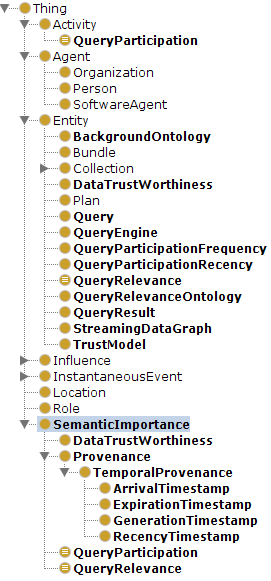
\includegraphics[width=2.5in]{img/app-sio.png}
    \caption{\textbf{Semantic Importance Ontology Class Hierarchy}}
    \label{fig:app-sio}
\end{figure}

%
\section{SIO Class Definitions}
Figure \ref{fig:app-sio} shows the class hierarchy in SIO.
SIO imports Prov-O ontology, and its own classes are in bold. 
SIO is designed as a descriptive ontology.

\begin{table}[!htbp]
    \centering
    \caption{\textbf{SIO Class Definition}}
    \begin{tabular}{|c||l|} \hline
         class name & \multicolumn{1}{c|}{definition}  \\ \hhline{|=#=|}
         QueryParticipation & \makecell[l]{(\textit{used some} \textbf{QueryEngine}) \textit{and} \\ (\textit{used some} \textbf{StreamingDataGraph}) \textit{and} \\(\textit{used some} \textbf{BackgroundOntologyFile}) \textit{and} \\(\textit{generated some} \textbf{QueryResult})} \\ \hline 
         QueryRelevance & \textit{wasDerivedFrom some} \textbf{QueryRelevanceOntologyFile} \\ \hline
        \multicolumn{2}{|l|}{\makecell{other classes do not need to be defined with OWL since they are not \\compound concepts, and can be described in natural languages.}} \\ \hline
    \end{tabular}
    \label{tab:app-socd}
\end{table}

Table \ref{tab:app-socd} shows the class OWL definitions.
Both \textbf{QueryParticipation} and \textbf{QueryRelevance} are compound classes, thus needs to be defined in OWL with clear semantics. 
Other classes do not have to be defined in OWL as they can be described in natural languages. 
%
\section{SIO Class Instances}
This section covers the grounded instances for each class in SIO.
Table \ref{tab:app-gi} shows the all instances for each class. 
These instances are self-explanatory by their names.
This section will only highlight some discussions.

\textbf{DataTrustworthiness} class has a concrete instance of \textit{left\_foot\_position\_is\\\_trusted\_right\_foot\_position\_is\_untrusted}.
Chapter 5 has mentioned that Player B4's sensor is likely to fail.
This observation leads to this simple data trustworthiness model, which essentially only trusts left foot position. 
Of course more sophisticated trust models are welcome, the point is to show an example of the trust model. 
Developing a trust model is out of the realm of this dissertation.

The instance of \textbf{Query} is \textit{who\_commits\_an\_offside\_offence}. 
When deployed in the system, this instance is a physical continuous query file that can be loaded in the system, such as CSPARQL or CQELS queries. 
\textbf{QueryEngine} indicates what triple-store and SPARQL query engine that the system uses. 
In this case, Stardog is used. 
Nonetheless, any other database will be the instance of \textbf{QueryEngine} if used. 

\textbf{QueryParticipationFrequency} describes how many times the data participates in the query during its time-to-live.
When deployed in the system, it is an integer value that can be used to rank the data. 

\textbf{StreamingDataGraph} class describes the actual RDF streaming data.
In this case, each triple is encapsulated in a unique graph, which makes it easier to manage the data.
In fact, a graph can contain multiple streaming data items. 
An example is to use the streaming source as the graph ID and all the generated data items are within this graph. 

\begin{center}
\begin{longtable}{|c||c||c|}
	\caption{\textbf{SIO Class Instances}} \label{tab:app-gi} \\
	\hline \multicolumn{1}{|c||}{class name} & \multicolumn{1}{c||}{instance example} & \multicolumn{1}{c|}{annotation} \\ \hhline{|=#=#=|}
	\endfirsthead
	\multicolumn{3}{c}%
	{{\bfseries \tablename\ \thetable{} -- continued from previous page}} \\
	\hline \multicolumn{1}{|c||}{class name} &
	\multicolumn{1}{c||}{instance example} &
	\multicolumn{1}{c|}{annotation} \\ \hline 
	\endhead
	\hline \multicolumn{3}{|r|}{{Continued on next page}} \\ \hline
	\endfoot
	\hline
	\endlastfoot
	\makecell{Background\\OntologyFile} & \makecell{soccer\_offside\_\\background\_ontology} & \makecell[l]{soccer offside background ontology \\ provides necessary knowledge \\ for defining \& determining \\soccer offside.} \\ \hline
	\makecell{DataTrust-\\worthiness} & \makecell{right\_foot\_position\_\\is\_trusted\_\\left\_foot\_position\_\\is\_untrusted} & \makecell[l]{right foot position is trusted, \\left foot position is not trusted} \\ \hline
	Query & \makecell{who\_commits\_an\_\\offside\_offence} & \makecell[l]{the query ``who commits an offside \\offence'' is the target query and \\registered in the system} \\ \hline
	QueryEngine & \makecell{stardog\_triplestore\_\\SPARQL\_engine} & \makecell[l]{in soccer offside use case, Stardog \\triplestore is used thus its SPARQL \\query engine is used.} \\ \hline
	\makecell{Query\\Participation\\Frequency} & \makecell{graph1\_query\_\\participation\_\\frequency\_value} & \makecell[l]{graph1 refers to\\``graph1\_PlayerA\_a\_Attacker''\\ (see StreamingDataGraph \\individuals for details)} \\ \hline
	\makecell{Query\\Participation\\Recency} & \makecell{graph1\_query\_\\participation\_\\recency\_timestamp} & \makecell[l]{the timestamp when graph1 \\participates in the query.} \\ \hline
	\makecell{Query\\Relevance\\OntologyFile} & \makecell{soccer\_offside\_query\_\\relevance\_ontology} & \makecell[l]{the query relevance ontology to \\help filter irrelevant data out} \\ \hline
	\makecell{QueryResult} & \makecell{PlayerA\_commits\_\\an\_offside\_offence} & \makecell[l]{the query result indicates \\that PlayerA commits \\an offside offence} \\ \hline
	\makecell{Streaming\\DataGraph} & \makecell{graph1\_PlayerA\_a\_\\Attacker.\\graph2\_PlayerA\_a\_\\BallLastToucher.\\graph3\_PlayerA\_a\_\\PlayerAtOffsidePosition.\\graph4\_PlayerB\_a\_\\Attacker.} & \makecell[l]{``graph1\_PlayerA\_a\_Attacker'' \\indicates that the triple \\``PlayerA a Attacker''\\ is in graph1. In this example, \\every graph only has 1 triple. \\(It could have more, \\but we set it to only have 1)} \\ \hline
	TrustModel & \makecell{left\_foot\_position\_\\has\_trust\_score\_\\of\_1\_right\_has\_0} & \makecell[l]{trust model stamps \\trust scores to data} \\ \hline
	\makecell{Arrival\\Timestamp} & \makecell{graph1\_arrival\_\\timestamp} & \makecell[l]{the arrival timestamp of graph1} \\ \hline
	\makecell{Expiration\\Timestamp} & \makecell{graph1\_expiration\_\\timestamp} & \makecell[l]{the expiration timestamp of graph1} \\ \hline
	\makecell{Generation\\Timestamp} & \makecell{graph1\_generation\_\\timestamp} & \makecell[l]{the generation timestamp of graph1} \\ \hline
	\makecell{Recency\\timestamp} & \makecell{graph1\_query\_\\participation\_recency\_\\timestamp} & \makecell[l]{the most recent query participation\\ timestamp of graph1} \\ \hline
	\makecell{Query\\Participation} & \makecell{graph1\_graph2\_graph3\_\\background\_ontology\_\\stardog\_query\_engine\_\\target\_query\_\\query\_result} & \makecell[l]{please refer to Table \ref{tab:app-socd}} \\ \hline
	\makecell{Query\\Relevance} & \makecell{graph1\_is\_relevant\_\\to\_query\\graph7\_is\_irrelevant\_\\to\_query} & \makecell[l]{the relevance is determined \\by the query relevance ontology} \\
\end{longtable}
\end{center}
%
\section{Instance Property Assertions}
Instances are inter-related.
This relationship is established via properties. 

\begin{center}
\begin{longtable}{|c||c||c|}
\caption{\textbf{SIO Instance Property Assertions}} \label{tab:app-ipa} \\

\hline \multicolumn{1}{|c||}{\textbf{Class Name}} & \multicolumn{1}{c||}{\textbf{Instance Example}} & \multicolumn{1}{c|}{\textbf{Property Assertion}} \\ \hhline{|=#=#=|}
\endfirsthead

\multicolumn{3}{c}%
{{\bfseries \tablename\ \thetable{} -- continued from previous page}} \\
\hline \multicolumn{1}{|c||}{\textbf{Class Name}} &
\multicolumn{1}{c||}{\textbf{Instance Example}} &
\multicolumn{1}{c|}{\textbf{Property Assertion}} \\ \hline 
\endhead

\hline \multicolumn{3}{|r|}{{Continued on next page}} \\ \hline
\endfoot

\hline
\endlastfoot
\makecell{DataTrust-\\worthiness} & \makecell{left\_foot\_position\_\\is\_trusted\_\\right\_foot\_position\_\\is\_untrusted} & \makecell{object property assertion: \\wasDerivedFrom \\ left\_foot\_position\_\\has\_trust\_score\_\\of\_1\_right\_has\_0\\ data property assertion: \\value 10} \\ \hline
\makecell{Query\\Participation\\Frequency} & \makecell{graph1\_query\_\\participation\_\\frequency\_value} & \makecell{data property assertion: \\value 3} \\ \hline
\makecell{Query\\Participation\\Recency} & \makecell{graph1\_query\_\\participation\_\\recency\_timestamp} & \makecell{data property assertion: \\value ``2011-07-16T02:52:02Z''\\\string^\string^dateTime } \\ \hline
\makecell{Arrival\\Timestamp} & \makecell{graph1\_arrival\_\\timestamp} & \makecell{data property assertion: \\value ``2011-08-16T02:52:02Z''\\\string^\string^dateTime } \\ \hline
\makecell{Expiration\\Timestamp} & \makecell{graph1\_expiration\_\\timestamp} & \makecell{data property assertion: \\value ``2011-09-16T02:52:02Z''\\\string^\string^dateTime } \\ \hline
\makecell{Generation\\Timestamp} & \makecell{graph1\_generation\_\\timestamp} & \makecell{data property assertion: \\value ``2011-10-16T02:52:02Z''\\\string^\string^dateTime } \\ \hline
\makecell{Recency\\timestamp} & \makecell{graph1\_query\_\\participation\_recency\_\\timestamp} & \makecell{data property assertion: \\value ``2011-11-16T02:52:02Z''\\\string^\string^dateTime } \\ \hline
\makecell{Query\\Participation} & \makecell{graph1\_graph2\_graph3\_\\background\_ontology\_\\stardog\_query\_engine\_\\target\_query\_\\query\_result} & \makecell{object property assertion: \\generated PlayerA\_commits\_an\_\\offside\_offence; \\used graph1\_PlayerA\_\\a\_attacker; \\used stardog\_triplestore\_\\sparql\_engine; \\generated graph1\_query\_\\participation\_frequency\_\\value; \\generated graph1\_query\_\\participation\_recency\_\\timestamp; \\used soccer\_offside\_\\background\_ontology; \\used graph2\_PlayerA\_\\a\_BallLastToucher; \\used graph3\_PlayerA\_\\a\_PlayerAtOffsidePosition} \\ \hline
\makecell{Query\\Relevance} & \makecell{graph1\_is\_relevant\_\\to\_query\\graph7\_is\_irrelevant\_\\to\_query} & \makecell{object property assertion: \\ wasDerivedFrom soccer\_offside\_query\_\\relevance\_ontology} \\
\end{longtable}
\end{center}
%
\section{Described Examples}
This section shows some concrete examples for selected classes and instances. 
\subsection{Query Participation Example}
Data items participate in a query if they contain necessary information used by the query engine to return non-empty answers.
When a data item particpates in a query, related meta-data such as the timestamp and frequency value can be collected. 
Consider a snapshot of streaming data as follows:

\begin{lstlisting}[caption={\textbf{Example Streaming Data}},basicstyle=\small]
PlayerA a Attacker, graph1
PlayerA a BallLastToucher, graph2
PlayerA a PlayerAtOffsidePosition, graph3
PlayerB a Attacker, graph4
PlayerB hasPosition LeftFootPosition, graph5
PlayerB hasPosition RightFootPosition, graph6
PlayerC a Defender, graph7
\end{lstlisting}

In this use case, Stardog SPARQL engine is used as the \textbf{QueryEngine},  \textbf{BackgroundOntology} encodes that a player who commits an offside offence should be: (i) \textit{player rdf:type} \textbf{Attacker}, (ii) \textit{player rdf:type} \textbf{BallLastToucher}, and (iii) \textit{player rdf:type} \textbf{PlayerAtOffsidePosition}.
For the streaming data in Listing A.1; graph1 contains Triple i; graph2 contains Triple ii; graph3 contains Triple iii; graph4 contains Triple i; graph5 does not convey Triple i, ii, or iii; graph6 does not convey Triple i, ii, or iii; graph7 does not convey Triple i, ii, or iii.
Thus, a \textbf{QueryResult} is given: Player A commits an offside offence. 
According to \textbf{QueryParticipation} class definition in Table \ref{tab:app-socd}, the streaming data graphs used to generate the query result are said to have participated in the query. 
Thus: graph1, graph2, \& graph3 have successfully participated in the query, while graph4, graph5, graph6, \& graph7 have unsuccessfully participated in the query.

Graph1, graph2, \& graph3's frequencies and recency will be updated.
Graph4, graph5, graph6, \& graph7's frequencies and recency will not be updated. 
If ranked by query participation, then graph1, graph2, graph3 will rank equally on the top, and graph4, graph5, graph6, graph7 will rank equally at the bottom.
%